% AI+RES write-up: GenCast walkers, FourCastNet 3 score.
% Build (Derecho):  module load texlive/20250308 && latexmk -pdf aires_writeup.tex
% Trajectory PDFs are read in place from ../../figures/aires/ (top title band trimmed
% with includegraphics). The two map PNGs in figs/ are copies of
% figures/aires/PNW_HeatDome_2021/aires_{anom_maps,map_walk}_PNW_HeatDome_2021_pilot.png
% with the matplotlib suptitle band cropped off (magick -crop ... -trim); pixels otherwise
% unchanged.
\documentclass[10pt,twocolumn]{article}

\usepackage[letterpaper,margin=0.7in,columnsep=0.25in]{geometry}
\usepackage[T1]{fontenc}
\usepackage[utf8]{inputenc}
\usepackage{newtxtext,newtxmath}
\usepackage{microtype}
\usepackage{amsmath}
\usepackage{graphicx}
\usepackage{booktabs,array}
\usepackage{siunitx}
\usepackage{caption}
\usepackage{stfloats}
\usepackage{enumitem}
\usepackage{xcolor}
\usepackage[numbers,sort&compress]{natbib}
\usepackage[colorlinks=true,linkcolor=blue!50!black,citecolor=blue!50!black,urlcolor=blue!50!black]{hyperref}
\usepackage{doi}
\usepackage{cleveref}

\graphicspath{{../../figures/aires/}}
\sisetup{separate-uncertainty=true,range-phrase=--,range-units=single}
\captionsetup{font=small,labelfont=bf,skip=4pt}
\setlist{nosep,leftmargin=*}
\setlength{\parskip}{0pt}
\bibliographystyle{unsrtnat}
\renewcommand{\bibfont}{\footnotesize}
\setlength{\bibsep}{3pt}

% Let two full-width figures share a page instead of stranding one per page.
\renewcommand{\dbltopfraction}{0.95}
\renewcommand{\topfraction}{0.95}
\renewcommand{\textfraction}{0.05}
\renewcommand{\dblfloatpagefraction}{0.7}
\renewcommand{\floatpagefraction}{0.7}
\setcounter{dbltopnumber}{3}
\setcounter{topnumber}{3}

% Notation. One symbol, one meaning, across the document.
%   A_L         : the observable, L-day box-mean 2 m temperature anomaly at the peak
%   theta       : the score, an M-member FCN3 ensemble mean of A_L
%   V_k, C_k    : splitting function and its coefficient at barrier k
%   N, M, K     : walkers, score members, barriers;  n^i_k : copies of walker i at barrier k
%   tau         : barrier spacing
%   Z           : product of per-barrier mean weight factors (= wbar_K)
%   sigma-depth : (obs - direct mean)/direct sd on the direct GenCast ensemble
\newcommand{\AL}{A_L}
\newcommand{\Tm}{T_{2\mathrm{m}}}
\newcommand{\vk}{V_k}
\newcommand{\ck}{C_k}
\newcommand{\verify}[1]{{\color{red!70!black}[VERIFY: #1]}}

\title{\Large Rare-event sampling of subseasonal CONUS extremes with GenCast walkers and a FourCastNet~3 score function}
\author{Eric Xu\\[2pt]\normalsize Vayuh \verify{affiliation}}
\date{\normalsize \today\quad(draft)}

\begin{document}
\maketitle

\begin{abstract}
\noindent
An ensemble forecast of 24 members cannot resolve an event whose probability at the forecast lead is much below $1/24$, and at week~3 the temperature extremes over the contiguous United States (CONUS) studied here are such events. Lancelin et al.\ introduced AI+RES, a rare-event algorithm in which a physics model propagates a population of walkers and a fast machine-learning emulator scores each walker by its forecast of the observable, so that computation is concentrated on the trajectories most likely to produce the event. We port the algorithm to the subseasonal forecasting problem with two changes. The walker is GenCast at 0.25\si{\degree}, a stochastic diffusion model whose clones separate without an imposed perturbation, and the score is FourCastNet~3, an independently trained model joined to the walker through a 72-channel adapter. With 64 walkers, five resampling barriers and a fixed splitting schedule, the method reaches the observed 7-day box-mean anomaly on six of the seven hindcast events that lie at least 1.9 standard deviations into the tail of a direct ensemble of 16 to 24 members at 21-day lead, including two winter freezes. The direct ensemble reaches it on one of the seven, with one member. On the one event where it was run, the same configuration with the walker's current anomaly as the score reaches the observed value with 0 of 64 walkers. Where direct sampling can resolve a probability and the resampled population still straddles the target, the weighted estimate agrees with it. We describe the algorithm, the implementation, the trajectory of every walker for four events, and the calibration campaign and hurricane score now in progress.
\end{abstract}

\section{Why sample rare events at all}
\label{sec:why}

A forecast ensemble estimates the probability of an event by counting the members that produce it. With $n$ members the smallest probability that can be distinguished from zero is of order $1/n$, and a single member landing on the event is indistinguishable from chance. The Pacific Northwest heat dome of June 2021 is the standard example. Its 7-day mean 2 m temperature anomaly over a 6\si{\degree} box covering the Pacific Northwest (\cref{tab:slate}) was \SI{+7.72}{K} in the ERA5 reanalysis of the European Centre for Medium-Range Weather Forecasts \citep{hersbach2020era5}. A 24-member GenCast ensemble \citep{price2025gencast} initialised 21 days before the peak places that value about two standard deviations above its mean and produces zero members that reach it (\cref{tab:slate}). The operational Climate Forecast System version 2 (CFSv2) \citep{saha2014cfsv2} at the same lead has an ensemble mean of \SI{+0.30}{K}. The forecast distribution may well carry a few percent of its mass at the observed value, but no affordable ensemble can say so.

Rare-event sampling (RES) estimates such probabilities at a fraction of the cost of a direct ensemble. Trajectories are run in parallel, periodically ranked by a score, and the population is resampled toward the high-scoring ones while a set of weights keeps the estimated probabilities unbiased \citep{delmoral2005genealogical,ragone2018heatwaves}. The long-standing obstacle is the score. In climate applications it has usually been the current value of the observable itself, which for a heat wave three weeks out carries no information about which walkers will become hot. \citet{lancelin2026airres} resolve this by letting a machine-learning weather emulator forecast each walker's future and using that forecast as the score. This note describes that algorithm, what changes when both the walker and the scorer are machine-learning weather models trained on reanalysis, and what the resulting system does on nine hindcast events.

\section{The AI+RES algorithm}
\label{sec:algo}

\citet{lancelin2026airres} study midlatitude heat waves in the PlaSim general circulation model. The observable is the $L$-day mean of 2 m temperature over a region $R$,
\begin{equation}
  \AL(t) = \frac{1}{L}\int_{t}^{t+L}\frac{1}{|R|}\int_{R} \Tm(\mathbf{r},s)\,\mathrm{d}\mathbf{r}\,\mathrm{d}s ,
  \label{eq:AL}
\end{equation}
with $L = 7$ days, and the quantity of interest is $P[\AL(t_f) > a]$ at a fixed target time $t_f$ for large thresholds $a$. Every value of $\AL$ reported in this note is an anomaly, the 2 m temperature minus the 1990 to 2019 ERA5 climatology on the same grid and hour. The discrete index averages the 13 twelve-hourly frames on the seven calendar days from $t_f$ to the event peak, a span of $6\times 24$ h inclusive of both endpoints. $L = 7$ d is the paper's nominal value and is kept here.

\paragraph{Walkers and barriers.}
$N$ copies of the model, the walkers $X^i_t$, are integrated in parallel from perturbed initial conditions. At resampling times $t_1 < \dots < t_K = t_f$, spaced $\tau$ apart and called barriers below, each walker receives a scalar score $\theta(X^i_k)$ and a splitting function
\begin{equation}
  \vk(X^i_k) = \ck\,\theta(X^i_k),
  \label{eq:V}
\end{equation}
where $\ck \ge 0$ sets how hard the population is pushed at barrier $k$. The score is rescaled across the live population before \cref{eq:V} is applied, so one schedule of $\ck$ serves observables with different units and spreads. The paper's general scheme maps the empirical distribution of $\theta$ onto a Gaussian by a quantile transform, but at the population sizes it uses it rescales by the z-score across the live population instead. This implementation does the same.

\paragraph{Weights and resampling.}
The scheme is a Diffusion Monte Carlo (DMC) importance-splitting algorithm. Each walker carries a weight, updated at barrier $k$ from the change in the splitting function along the leg it has just travelled,
\begin{equation}
  w^i_k = \bar w_{k-1}\,\exp\!\big[\vk(X^i_k) - V_{k-1}(\hat X^i_{k-1})\big],
  \qquad
  \bar w_k = \frac{1}{N}\sum_{i=1}^{N} w^i_k ,
  \label{eq:w}
\end{equation}
where $\hat X^i_{k-1}$ is the state the walker was resampled from at the previous barrier, $V_0 = 0$ and hence $\bar w_0 = 1$. The population is then resampled. Walker $i$ is replaced by $n^i_k$ copies with $\sum_i n^i_k = N$ and $\mathbb{E}[n^i_k] = w^i_k/\bar w_k$, so a walker with twice the average weight expects two children and one with a small weight is likely to be killed. The copy counts are drawn by pivotal sampling \citep{deville1998pivotal}, which fixes the total at exactly $N$ while preserving each marginal. The selected walkers are integrated to the next barrier and the step repeats.

\paragraph{The estimator.}
Because $V$ is a function of state alone, the weight factors telescope along any surviving lineage and the population after the last barrier is distributed under the tilted law $e^{V_K}\,\mathrm{d}P / \mathbb{E}_P[e^{V_K}]$. An expectation under the original forecast distribution $P$ is recovered by undoing the tilt,
\begin{equation}
  \mathbb{E}_P[\psi] \approx Z\,\frac{1}{N}\sum_{i=1}^{N}\psi(X^i)\,e^{-V_K(\text{lineage of } i)},
  \label{eq:est}
\end{equation}
where $V_K(\text{lineage of } i)$ is the splitting function of walker $i$'s ancestor at the last barrier and
\begin{equation}
  Z = \prod_{k=1}^{K}\frac{1}{N}\sum_{i=1}^{N} e^{\vk(X^i_k)-V_{k-1}(\hat X^i_{k-1})} = \bar w_K
  \label{eq:Z}
\end{equation}
is the running mean weight of \cref{eq:w} after the last barrier. \Cref{eq:est} is Eq.~(2) of \citet{lancelin2026airres} evaluated after the last barrier, with $\bar w_K$ written as a product. Taking $\psi = \mathbf{1}\{\AL \ge a\}$ gives the exceedance curve $P[\AL \ge a]$ for every $a$ at once. Taking $\psi \equiv 1$ gives
\begin{equation}
  \hat 1 = Z\,\frac{1}{N}\sum_{i=1}^{N} e^{-V_K(\text{lineage of } i)},
  \label{eq:norm}
\end{equation}
which equals one in expectation for deterministic $V$ and is called the normalisation check in \cref{sec:results}. Setting every $\ck = 0$ makes $V \equiv 0$, $Z = 1$ and every weight one, so the algorithm reduces to direct sampling. The estimator is unbiased when $V$ is deterministic. The population rescaling of the score makes the walkers interact and weakens the guarantee to consistency.

\paragraph{The score.}
The step that makes the algorithm AI+RES is the choice of $\theta$. At each barrier and for each walker, an $M$-member ensemble forecast is run with a fast emulator from the walker's current state to the target window, and the score is the ensemble mean of the forecast observable,
\begin{equation}
  \theta(X^i_k) = \frac{1}{M}\sum_{j=1}^{M}\hat A^{\,i,j}_L(t_f \,|\, X^i_k).
  \label{eq:theta}
\end{equation}
This favours cloning walkers with a large conditional expectation of $\AL(t_f)$, without committing to a threshold $a$ in advance. The emulator in \citet{lancelin2026airres} is a deterministic neural network trained on 100 years of PlaSim output, run as an ensemble of $M = 100$ forecasts per walker generated by perturbing the initial condition.

\paragraph{What it bought.}
With $N = 400$ walkers, $K = 6$ barriers at $\tau = 5$ days and $\ck = (0,0,0,1.6,1.8,2.0)$, AI+RES reproduced return periods for heat waves over France and the U.S.\ Midwest out to 50\,000 years against a direct-sampling reference of $N = 50\,000$, a sampling speedup above 100 at a return period of $10^4$ years. The France variance speedup is the exception, peaking near 25 at about 2500 years and falling to 10 for the rarest events. The same algorithm with the traditional persistence score, called Standard-RES in the paper, saturates at return periods beyond about 100 years because it never selects the trajectories that later become extreme. The paper's discussion notes that an emulator trained probabilistically would let the score explore several plausible pathways to the event, and the framework should suit the tails of subseasonal-to-seasonal ensemble forecasts, where large ensembles are needed. That a stochastic model also removes the need to perturb clones by hand is our addition.

\section{Why it is useful here}
\label{sec:useful}

The subseasonal problem is the single-forecast version of the paper's climatological one. Instead of asking how often a 7-day anomaly exceeds $a$ in a stationary climate, we ask, for one initial condition at 21-day lead, how much of the forecast distribution lies beyond the anomaly that was later observed. The same estimator answers both. What the rare-event method adds over a larger ensemble is efficiency in the tail. The variance reduction of importance splitting grows with the depth of the target, so at a fixed budget it resolves probabilities a direct ensemble of equal cost cannot, while the weights of \cref{eq:est} keep the estimate on the same footing as a direct count wherever both can be measured. The resampled population is also a set of complete, physically consistent trajectories enriched in those that reach the event, so it can be composited and studied as a catalogue of pathways, which a tail of zero or one direct members does not supply.

\section{This implementation, and how it differs}
\label{sec:impl}

\begin{table}[t]
\centering\footnotesize
\caption{The configuration of \citet{lancelin2026airres} against this work. Cost is the range over the nine events of \cref{tab:slate} at $N = 64$ on one node of eight H100 GPUs.}
\label{tab:diff}
\begin{tabular}{@{}>{\raggedright\arraybackslash}p{2.0cm}>{\raggedright\arraybackslash}p{2.95cm}>{\raggedright\arraybackslash}p{2.95cm}@{}}
\toprule
 & Lancelin et al. & this work \\
\midrule
walker & PlaSim, deterministic & GenCast 0.25\si{\degree}, stochastic \\
scorer & emulator trained on PlaSim output & FourCastNet~3, trained on ERA5 \\
walker--scorer join & shared state space & 72-channel adapter \\
clone separation & log-$p_s$ perturbation, amplitude $3\times10^{-3}$ & diffusion noise \\
$N$ walkers & 400 & 64 \\
$M$ score members & 100 & 6 \\
$K$ barriers, $\tau$ & 6, 5 d & 5, 3 d \\
$\ck$ & $(0,0,0,1.6,1.8,2.0)$ & $(0,1.0,1.4,1.8,2.0)$ \\
$L$ & 7 d & 7 d \\
region $R$ & $3\times3$ grid points & event box, 6 to 12\si{\degree} on a side, or CONUS \\
target & return periods in a stationary climate & one hindcast at 21 d lead \\
reference & direct sampling, $N = 50\,000$ & ERA5 value and 16 to 24 direct members \\
cost per case & -- & 61 to \SI{64}{H100\,h}, 7.2 to \SI{8.7}{h} wall \\
\bottomrule
\end{tabular}
\end{table}

\Cref{tab:diff} lists the configuration side by side. The structural changes are the two models and the join between them.

\paragraph{A stochastic walker.}
GenCast \citep{price2025gencast} is a conditional diffusion model. Each 12 h step draws fresh noise, so two clones of one state diverge on their own. The paper's walker is deterministic and needs an explicit perturbation of the spherical harmonics of the logarithm of surface pressure after every resampling. We measured the separation the diffusion noise provides. Sibling clones born at the 15-day barrier differ by \SI{1.0}{K} root-mean-square 2 m temperature over CONUS after one 12 h step and by about \SI{2.5}{K} at the 21-day horizon, against \SIrange{3.0}{4.5}{K} for unrelated walkers. Clones separate, but at verification they are separated by only about 60\% of the unrelated-pair distance, so 64 resampled walkers hold fewer than 64 independent tail samples. The paper's perturbation is implemented and can be switched on if a later run resamples harder.

We use the 0.25\si{\degree} checkpoint trained on data before 2019, so every event studied is out of sample. One member peaks at about \SI{21}{GiB} of device memory in use and about \SI{113}{GB} of host memory. The walker runs one member per GPU because each process reserves 0.9 of the card as its JAX arena. A walker is rolled in segments, 3-day chunks that end at a barrier, and each segment writes a \SI{473}{MB} compressed global restart state, which brings the production rate to roughly \SI{52}{s} per 12 h step. That restart state is the price of a walker that can be stopped and cloned. The cached GenCast cubes of our earlier experiments are cropped to CONUS and cannot restart a walker, so the walker keeps a rolling two-frame global buffer and writes the CONUS crop separately.

\paragraph{An independent scorer.}
The score is FourCastNet~3 (FCN3) \citep{bonev2025fcn3}, a probabilistic 0.25\si{\degree} model with a 6 h step, run as $M = 6$ members from each walker's state to the target window. In the paper the emulator was trained on the walker's own output and is expressed in the walker's state space. Here the two models were trained separately on ERA5 and expose different variable sets, so a walker state has to be translated into an FCN3 initial condition. Of FCN3's 72 input channels, 69 are a rename of GenCast variables plus a latitude flip and are reproduced bit for bit. Three are derived. The 100 m winds come from a per-grid-point complex gain on the 10 m wind, fitted once against ERA5, and total column water vapour from a per-grid-point quadrature of the 13 humidity levels. On six held-out event dates the derived winds have a root-mean-square error of at worst \SI{0.63}{m\,s^{-1}} and the column water a relative error of at worst 4.6\%. An FCN3 ensemble started from an adapted ERA5 frame is indistinguishable from one started from FCN3's own native frame out to the 8.5-day predictability horizon of CONUS-mean $\Tm$, at every lead moving the forecast less than a change of random seed does. That test was run on one event at 24 members and resolves a shift in the mean observable no finer than about \SI{0.3}{K}.

Whether the score works is a separate question from whether the adapter is faithful, and it is the one that decides the experiment. The score does not have to be right about the atmosphere. It has to rank the walkers by where they themselves will end up, because that is all the resampling reads. We measured this on 16 free-running walkers of the 2021 heat dome, GenCast members rolled from the event's initial condition with no resampling, which also serve as a direct ensemble. With 16 walkers each correlation below carries a 95\% interval of roughly $\pm 0.3$. The Spearman correlation between $\theta$ at the barrier and the walker's own realised $\AL$ is $-0.04$ at 3 days, $0.61$ at 6, $0.80$ at 9, $0.96$ at 12 and $0.99$ at 15 days. The persistence score at the same leads is $-0.38$, $0.39$, $0.06$, $0.13$ and $0.56$. FCN3 is not reading the current state, and it acquires skill between 3 and 6 days, which is why $C_1 = 0$. The sampling error of a 6-member mean caps the attainable correlation at $0.95$ at 9 days and $0.99$ at 12, so $M = 6$ is not the binding constraint where resampling happens. The same gate was repeated for a south-central heat dome and for a Texas freeze, with FCN3 correlations of $0.70$/$0.77$ and $0.91$/$0.97$ at 9 and 12 days. For the south-central event persistence reaches $0.58$ at 12 days, so the margin over the current state is thin at that lead and it is the 9-day barrier, where persistence scores $-0.01$, that the FCN3 score pays for. For the freeze persistence is $0.43$ and $0.06$ at the two leads.

\paragraph{Schedule and observable.}
The five barriers are at leads 3, 6, 9, 12 and 15 days. The verification window is the seven calendar days ending at the event peak, leads 15 to 21 d, so $t_f = 15$ d and the horizon is 21 d. The $\ck$ schedule was chosen once by replaying the DMC loop on the measured skill curve and checking that the resampling effective sample size (ESS), the ESS of the weights $w^i_k$ at a barrier, does not collapse. It is not re-tuned per event, so whether one schedule generalises stays a testable statement. The region $R$ in \cref{eq:AL} is an event-centred box rather than the CONUS mean. For the 2021 heat dome the observed anomaly is \SI{+7.72}{K} over the Pacific Northwest box and \SI{+0.64}{K} over CONUS, and 13 of 16 free-running walkers already exceed the CONUS value, so a CONUS-mean experiment would have had no tail to find. For a cold event the sign of $\AL$ is flipped before scoring, so the sampler clones the most negative walkers.

\paragraph{What the result can claim.}
Inverting the paper's roles changes what is being sampled. There the walker was the high-fidelity reference and the emulator the cheap helper. Here the sampled distribution is GenCast's forecast distribution, not the atmosphere's, and the paper's own emulator-only baseline showed that machine-learning models have biased tails. The claim this experiment can support is that the method reaches the extreme tail of the GenCast forecast distribution efficiently and prices it consistently with direct sampling where the two overlap. It cannot support an unbiasedness claim against the real climate, and none is made in \cref{sec:results}.

\paragraph{Engineering.}
The walker is JAX and the scorer is PyTorch, in two conda environments that cannot share a process, so they hand off through disk. On one node the two pools alternate, because the JAX arena claimed for a resident GenCast and the roughly \SI{50}{GiB} FCN3 needs do not fit one \SI{80}{GB} card together. Resumption is replay rather than checkpointing. The loop is a deterministic function of the pivotal-sampling seed and the score cubes on disk, so a second pass reproduces every parent map and weight in seconds without a GPU, and a rewritten cube is an error rather than a silent fork. Retaining every global state would cost \SI{213}{GB} per event, so states more than two segments old are pruned. The diagnostics cubes every figure is drawn from are never pruned.

\section{Results on nine events}
\label{sec:results}

\begin{table*}[tp]
\centering\footnotesize\setlength{\tabcolsep}{4.5pt}
\caption{Nine hindcasts at 21-day lead, $N = 64$, $M = 6$, one fixed $\ck$ schedule. $\AL$ is the observed 7-day box-mean $\Tm$ anomaly in ERA5. $\sigma$-depth is its distance from the direct GenCast ensemble mean in units of that ensemble's standard deviation, signed so that positive is toward the event. The direct ensemble is the 24-member GenCast run, or the 16 free-running walkers for the south-central event. Direct and AI+RES columns count members reaching the observed value, with the most extreme member in parentheses. $P$ is the weighted estimate from \cref{eq:est}. The direct probability carries its Wilson 95\% interval. Rows are ordered by $\sigma$-depth. The last row is the persistence-score control for the 2021 heat dome.}
\label{tab:slate}
\begin{tabular}{@{}llS[table-format=+2.2]S[table-format=+1.2]llll@{}}
\toprule
event & box & {obs.\ $\AL$ (K)} & {$\sigma$-depth} & direct & AI+RES (64) & $P_{\text{AI+RES}}$ & $P_{\text{direct}}$ [95\%] \\
\midrule
Southwest heat wave, Aug 2020        & SW / S Plains     & +5.14  & 3.33 & 0/24 (+3.82)   & 0 (+4.31)    & $<3\times10^{-4}$ & 0 [0, 0.14] \\
California heat wave, Sep 2022       & California        & +4.71  & 2.85 & 0/24 (+4.70)   & 25 (+6.33)   & 0.019             & 0 [0, 0.14] \\
Winter Storm Elliott, Dec 2022       & N Plains          & -14.42 & 2.81 & 0/24 ($-9.83$) & 20 ($-17.04$) & 0.0079           & 0 [0, 0.14] \\
Winter Storm Uri, Feb 2021           & TX / OK           & -7.40  & 2.28 & 0/24 ($-6.51$) & 32 ($-10.20$) & 0.0090           & 0 [0, 0.14] \\
South-central heat dome, Jun 2023    & S Texas           & +5.73  & {$\approx$2.2$^a$} & 0/16 (+4.19)   & 6 (+6.19)    & 0.0027            & 0 [0, 0.19] \\
Pacific Northwest heat dome, Jun 2021 & Pacific Northwest & +7.72  & 1.98 & 0/24 (+7.08)   & 42 (+10.29)  & 0.054             & 0 [0, 0.14] \\
CONUS warm week, Dec 2025            & CONUS             & +3.26  & 1.91 & 1/24 (+3.46)   & 46 (+5.12)   & 0.066             & 0.042 [0.007, 0.20] \\
CONUS median week, Aug 2024          & CONUS             & +1.06  & 0.00 & 14/24 (+1.96)  & 63 (+2.37)   & 0.65              & 0.58 [0.39, 0.76] \\
CONUS below-median week, Nov 2023    & CONUS             & +0.21  & -0.97 & 21/24 (+3.14)  & 64 (+4.16)   & 0.58$^b$          & 0.88 [0.69, 0.96] \\
\midrule
Pacific Northwest, persistence score & Pacific Northwest & +7.72  & 1.98 & 0/24 (+7.08)   & 0 (+7.33)    & --                & 0 [0, 0.14] \\
\bottomrule
\end{tabular}
\par\smallskip
{\footnotesize $^a$~Recorded to one decimal only, against the 16 free-running walkers. $^b$~Pinned, because every walker lies past the target, so the estimator returns its own normalisation check and carries no information. See \cref{par:calib}.}
\end{table*}

\begin{figure*}[tp]
\centering
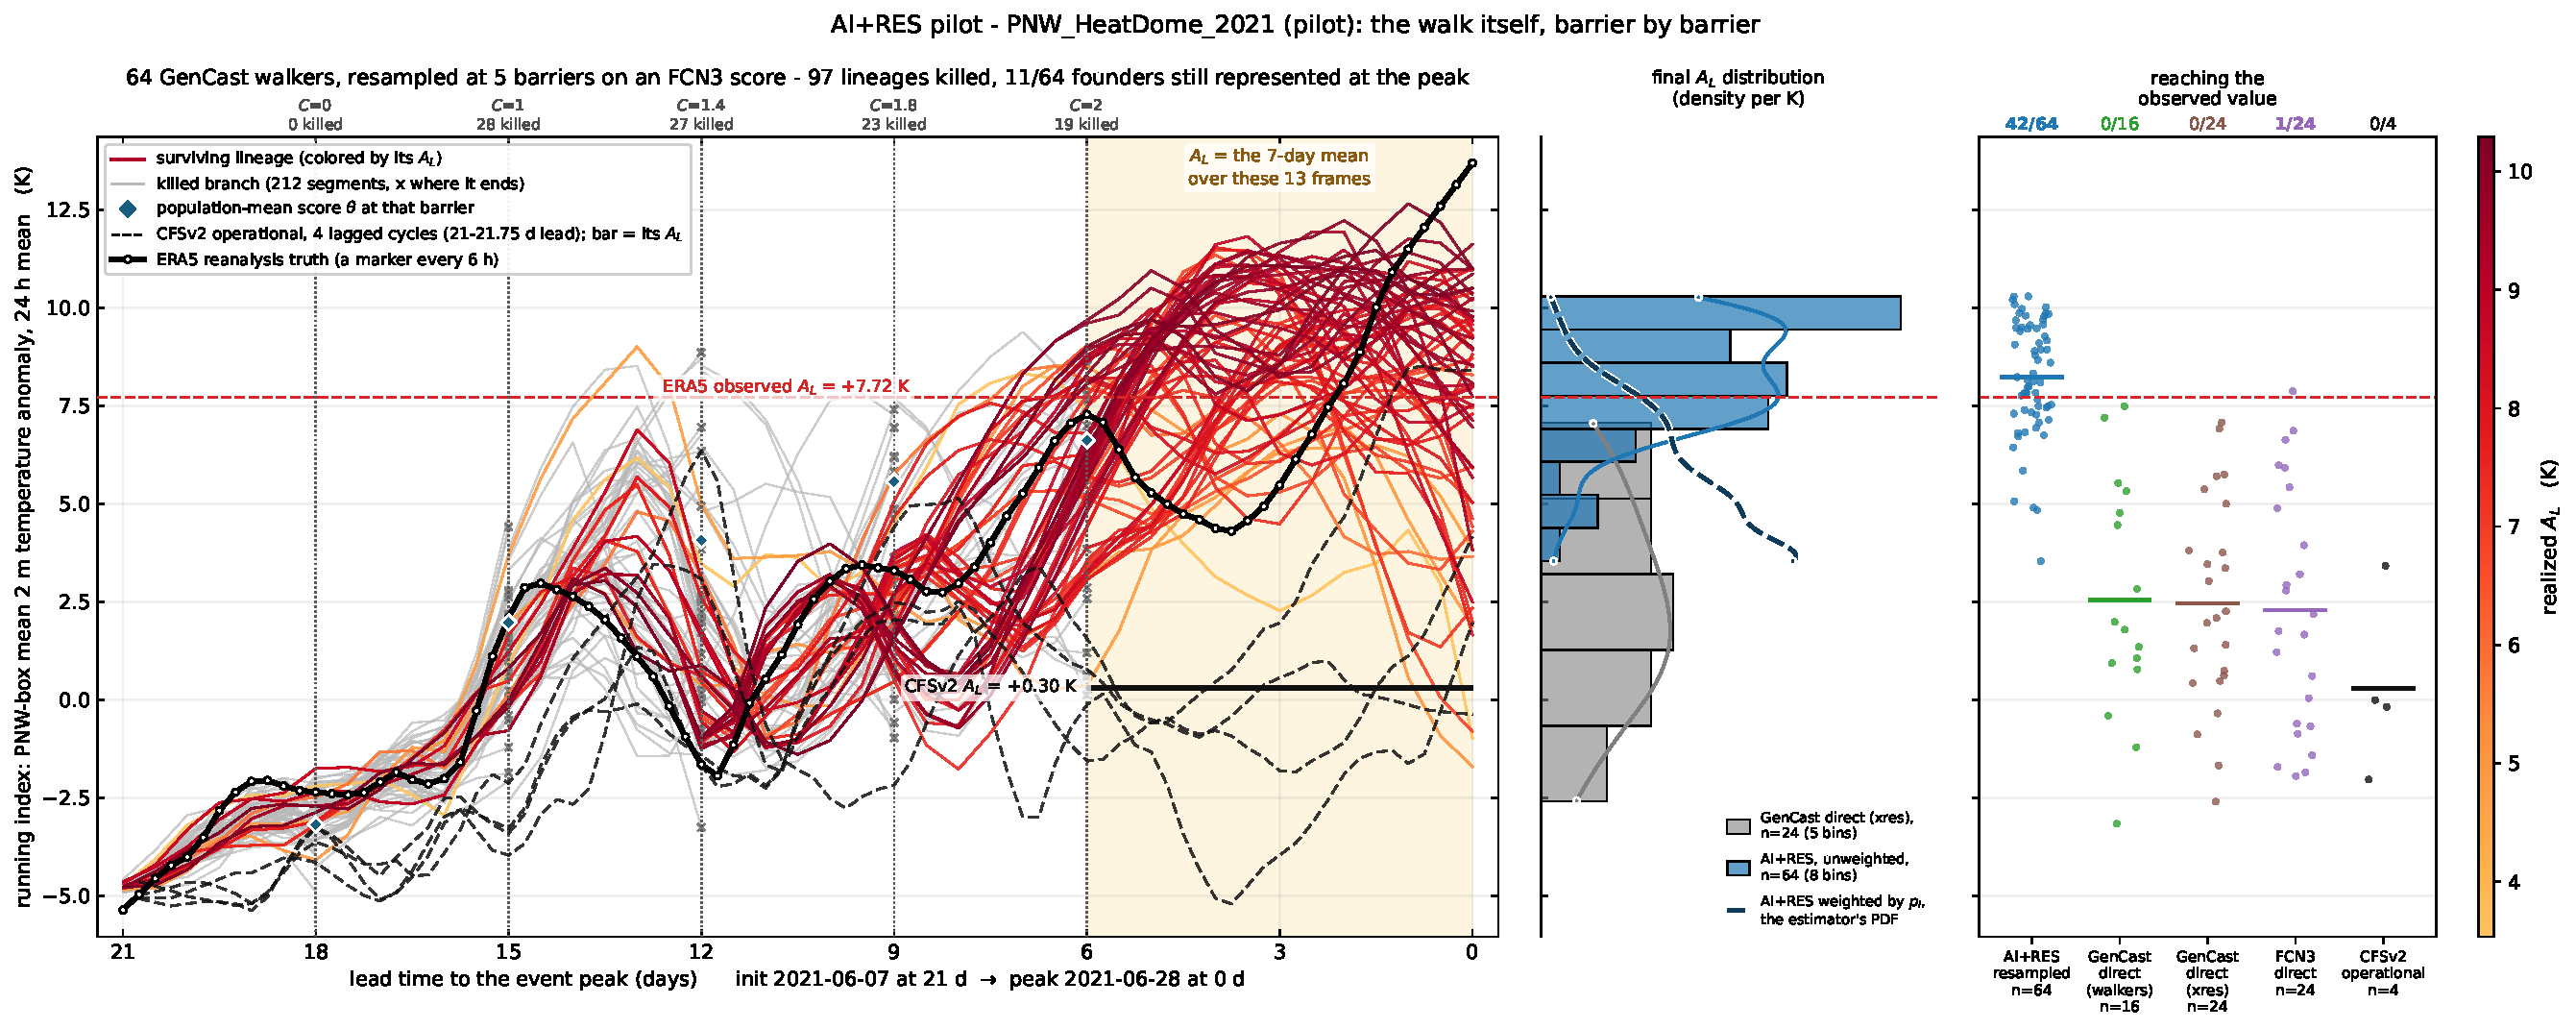
\includegraphics[width=\textwidth,trim=0 0 0 22,clip]{PNW_HeatDome_2021/aires_trajectory_PNW_HeatDome_2021_pilot.pdf}
\caption{The 2021 Pacific Northwest heat dome, 64 walkers, 21-day lead. Left, the running box-mean $\Tm$ anomaly (24 h mean) of every segment rolled. Grey branches were killed at a barrier. Coloured lineages survive to the peak and are coloured by their realised $\AL$. Dotted verticals are the five barriers, labelled by $\ck$ and by the number of lineages killed. Blue diamonds are the population-mean score $\theta$. The shaded band is the 7-day verification window over which $\AL$ is taken. The black line with markers is ERA5. Dashed black curves are the four lagged CFSv2 cycles at the same lead, with their mean $\AL$ as a bar. Middle, the distribution of final $\AL$ for the 24 direct GenCast members (grey), the unweighted resampled population (blue) and the weighted estimator (dashed). Right, where each method's members landed, with the count reaching the observed value above each column. The horizontal axis counts lead time down to the peak.}
\label{fig:traj_pnw}
\end{figure*}

\begin{figure*}[tp]
\centering
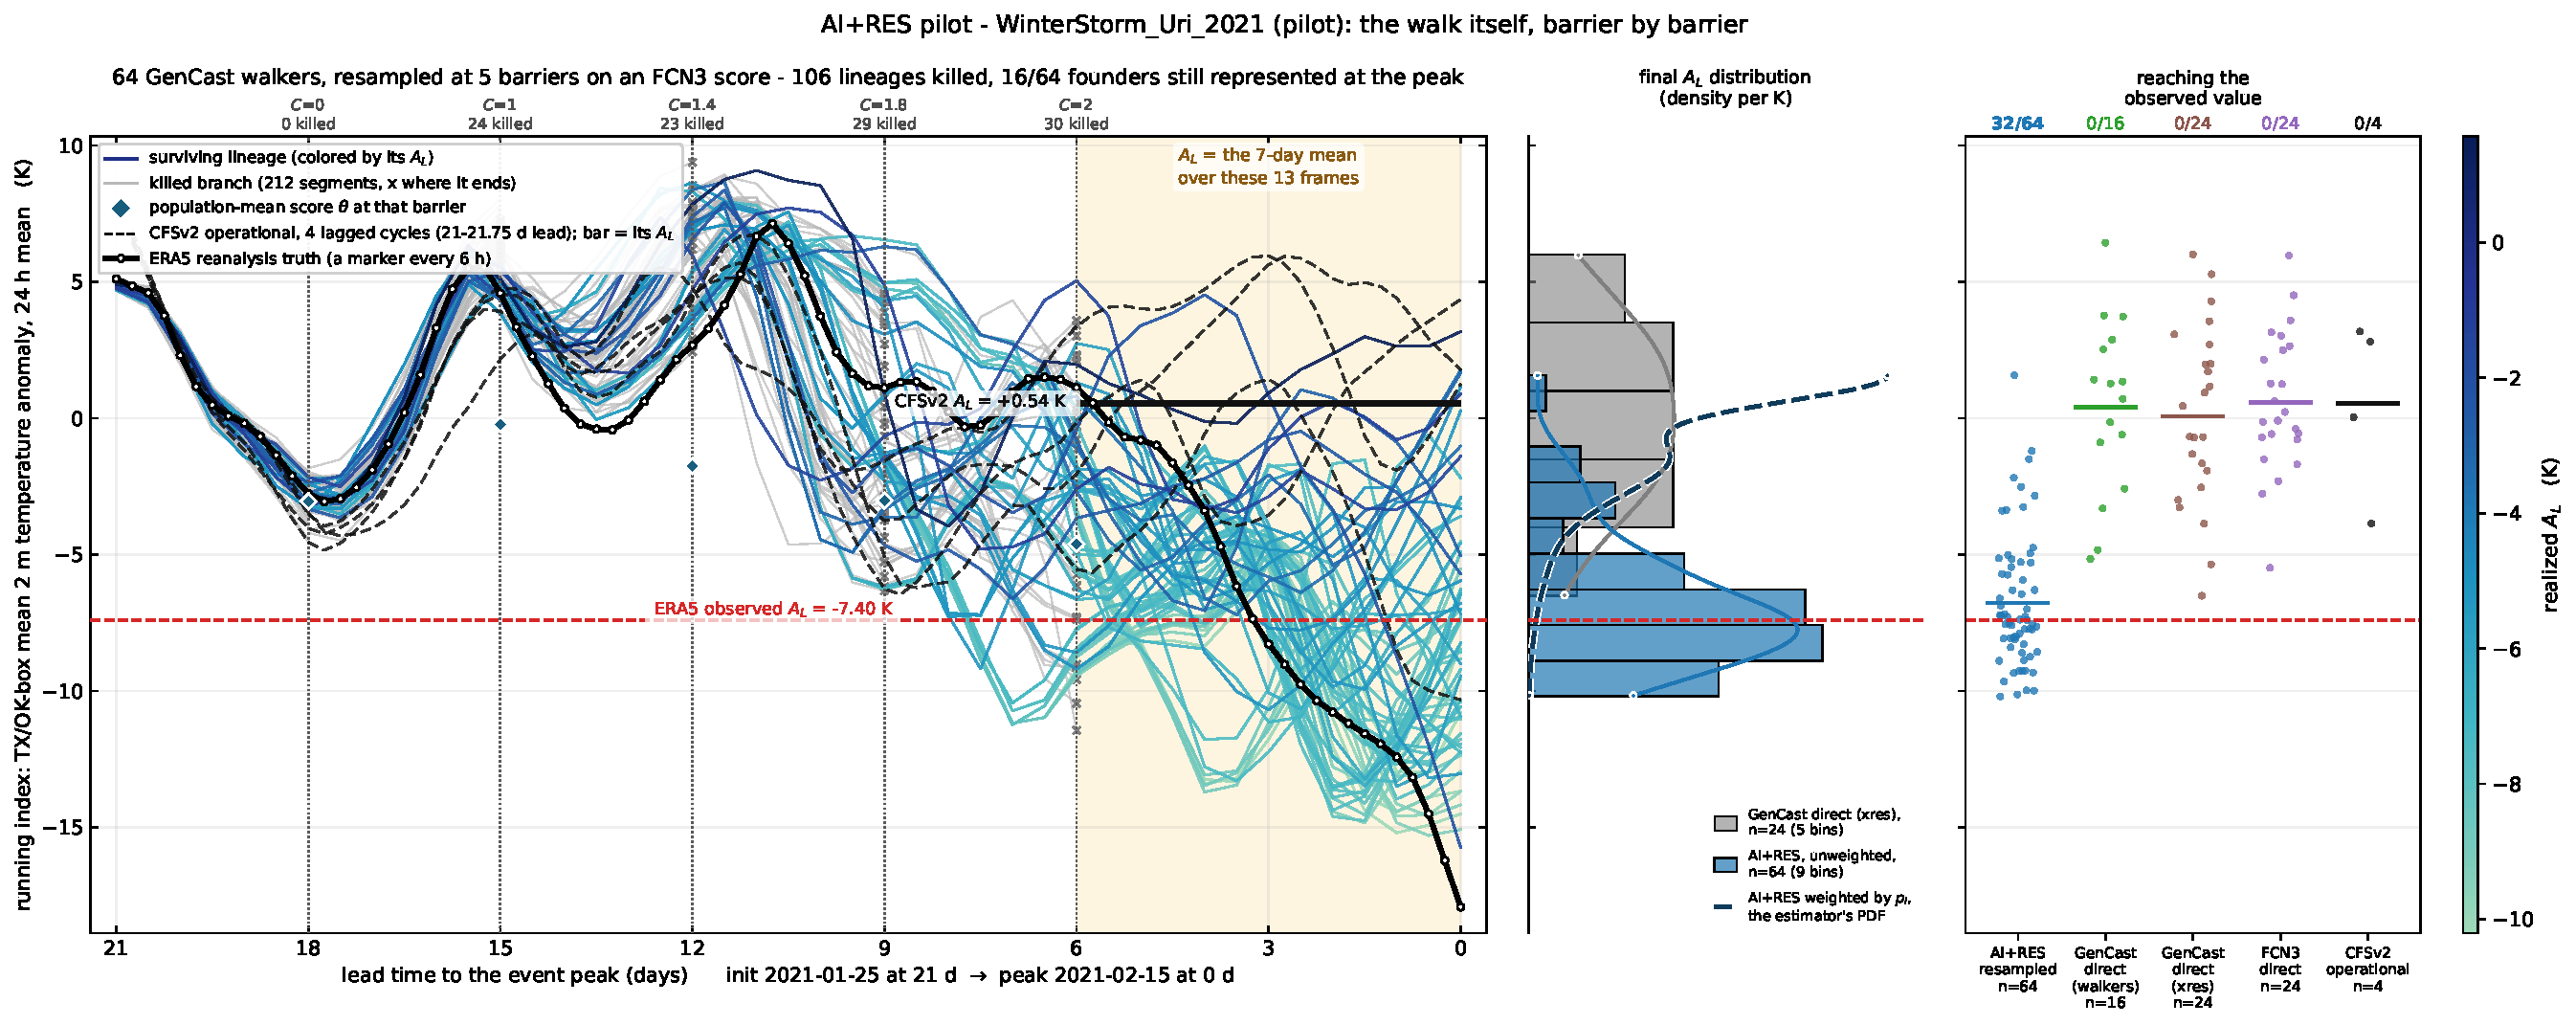
\includegraphics[width=\textwidth,trim=0 0 0 22,clip]{WinterStorm_Uri_2021/aires_trajectory_WinterStorm_Uri_2021_pilot.pdf}
\caption{As \cref{fig:traj_pnw}, for Winter Storm Uri, February 2021, over the Texas and Oklahoma box. The sign of $\AL$ is flipped before scoring, so the sampler clones the coldest walkers. The observed anomaly of \SI{-7.40}{K} is reached by 32 of 64 walkers, and the coldest reaches \SI{-10.20}{K}. None of 24 direct GenCast members, 16 free-running walkers or 24 direct FCN3 members reaches it.}
\label{fig:traj_uri}
\end{figure*}

\begin{figure*}[tp]
\centering
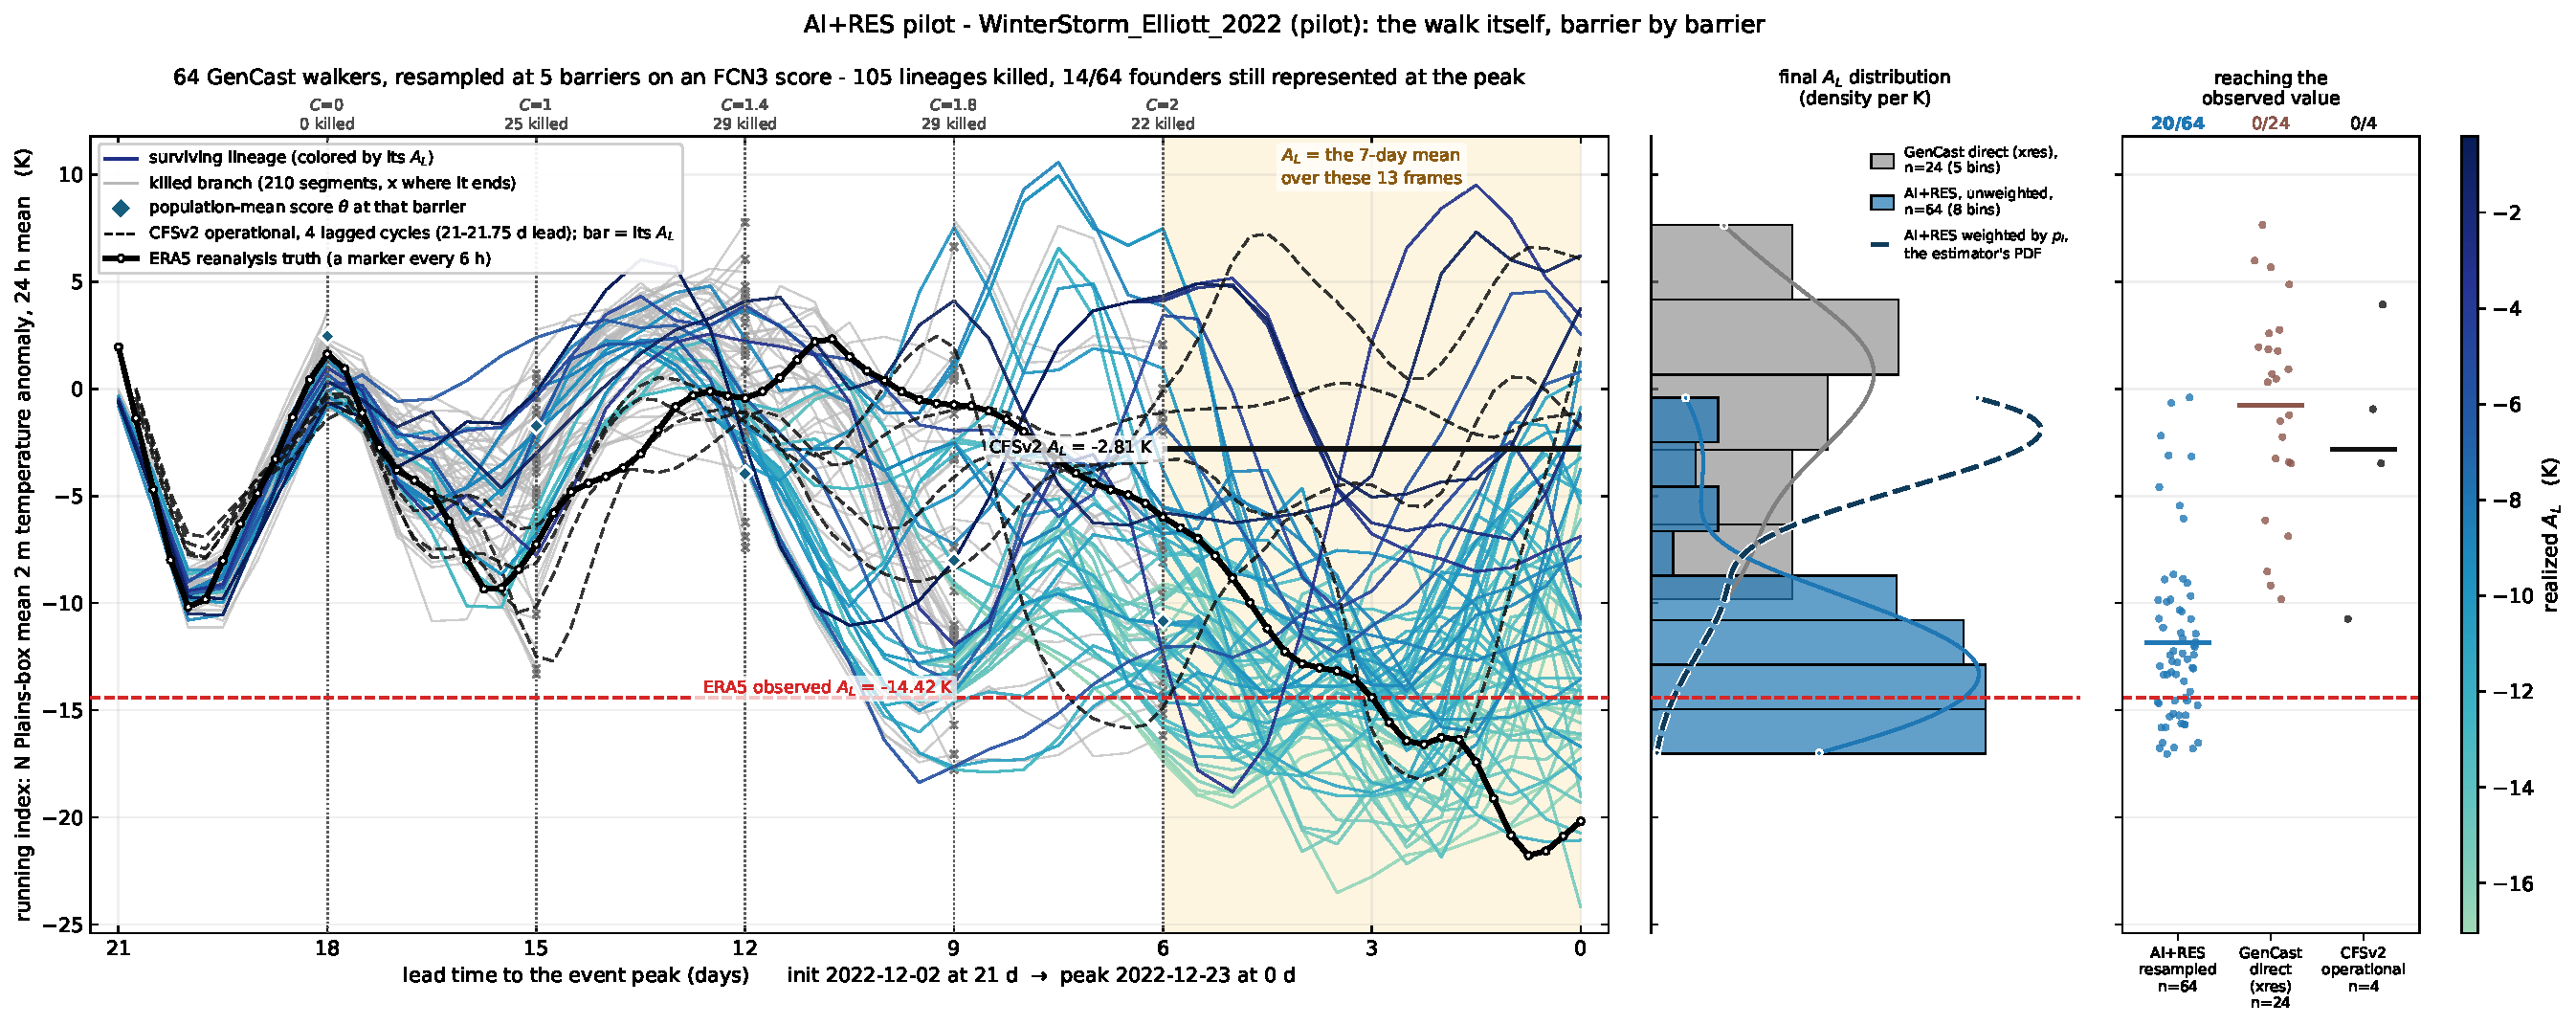
\includegraphics[width=\textwidth,trim=0 0 0 22,clip]{WinterStorm_Elliott_2022/aires_trajectory_WinterStorm_Elliott_2022_pilot.pdf}
\caption{As \cref{fig:traj_pnw}, for Winter Storm Elliott, December 2022, over the northern Plains box. At 2.81 standard deviations from the direct ensemble mean this is the deepest cold target reached in the experiment. The observed \SI{-14.42}{K} is reached by 20 of 64 walkers, where the coldest direct member stops \SI{4.6}{K} short.}
\label{fig:traj_elliott}
\end{figure*}

\begin{figure*}[tp]
\centering
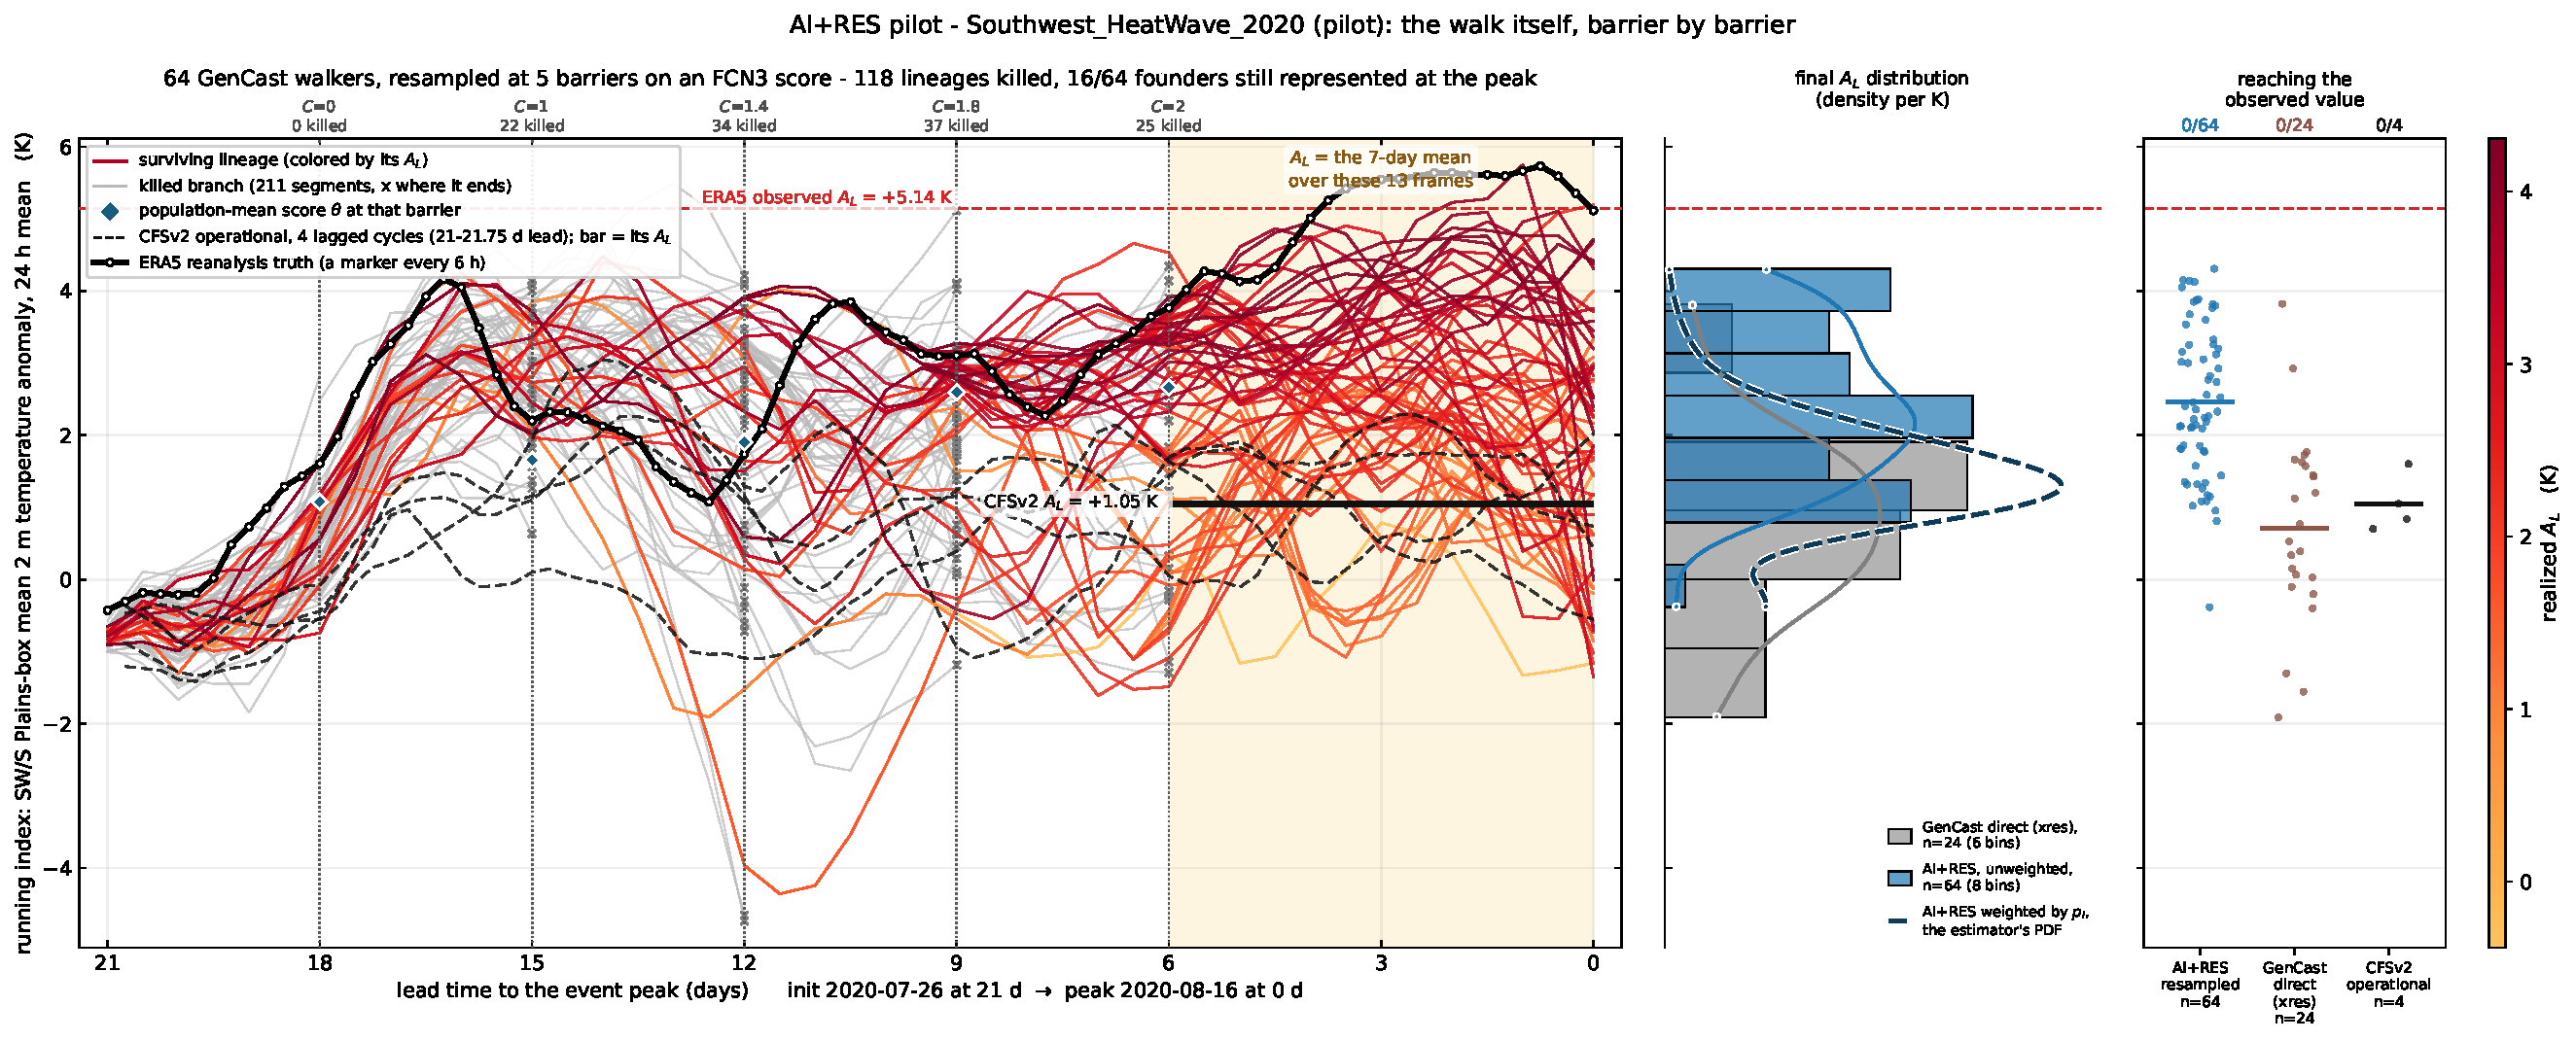
\includegraphics[width=\textwidth,trim=0 0 0 22,clip]{Southwest_HeatWave_2020/aires_trajectory_Southwest_HeatWave_2020_pilot.pdf}
\caption{As \cref{fig:traj_pnw}, for the August 2020 Southwest heat wave, the one target the run does not reach. The observation is 3.33 standard deviations above the direct mean. Resampling moves the population mean by about \SI{1.75}{K}, and the gap to the observation is \SI{4.4}{K}. Where direct sampling and the weighted estimate overlap they agree, so the miss is a limit of reach, not a failure of the weights.}
\label{fig:traj_sw}
\end{figure*}

\Cref{tab:slate} collects nine hindcasts. Each was run at $N = 64$ walkers, $M = 6$ score members and the same $\ck$ schedule, at 21-day lead. Each cost 61 to \SI{64}{H100\,h}, or 7.2 to \SI{8.7}{h} on one node of eight H100 GPUs. Events span four warm regional heat waves, two winter freezes and three CONUS-wide weeks chosen to lie at 1.9, 0.0 and $-1.0$ standard deviations from the direct ensemble mean, the last two as controls.

\paragraph{Reach.}
Where the observation lies between 1.98 and 2.85 standard deviations from the direct mean, AI+RES reaches it in every case, with between 6 and 42 of 64 walkers, while the direct ensemble reaches it in none. The two freezes are reached with a schedule ported unchanged from the warm events, so the result is not sign-dependent. The Southwest heat wave at 3.33 standard deviations is not reached (\cref{fig:traj_sw}). The reach boundary for this configuration therefore lies between 2.85 standard deviations (California, the deepest target reached) and 3.33 standard deviations of the walker's own forecast spread, and it is set by how far the model's distribution extends, not by the absolute anomaly. Elliott at \SI{-14.4}{K} is reached. The Southwest at \SI{+5.1}{K} is not.
% California's sigma-depth recomputed 2026-09-17 from runs/xres/0p25/week3/cache/California_HeatWave_2022_cube.nc
% with aires.aindex: mean +1.371, sd 1.172, max +4.700, obs +4.710 -> 2.849. PNW reproduces 1.981 by the same code.

\paragraph{The score is the ingredient.}
The last row of \cref{tab:slate} repeats the heat-dome run with the same walkers, the same barriers, the same seeds and the same $\ck$, replacing only the FCN3 score by the walker's current box anomaly, the Standard-RES score of \citet{lancelin2026airres}. It reaches the observed value with 0 of 64 walkers. Its selection is noise at these leads. The resampling ESS falls to 2 to 4\% of $N$ at the middle barriers, three founders survive, the weights span nearly five decades and the normalisation check of \cref{eq:norm} evaluates to 8.75 rather than near 1. Cloning on a skilful forecast of the event outperforms cloning on who is hottest now, which is what the gate correlations of \cref{sec:impl} predicted.

\paragraph{Calibration where it can be checked.}\label{par:calib}
A weighted probability is only checkable against a probability that direct sampling can resolve. The three CONUS-wide rows supply that. At 1.9 standard deviations the direct count is 1 of 24 and the weighted estimate of 0.066 lies inside its interval. At the ensemble median the plan predicted about 0.58 and the run returned 0.65, again inside. Both runs agree with direct sampling at the observation while running high through the middle of the curve, by about a factor of two on the December 2025 run, which is two to three binomial standard errors at 24 members and leans the same way at every threshold. Below the median the estimator fails. Resampling carried the whole population past a target of \SI{+0.21}{K} (the coolest walker finished at \SI{+1.50}{K}), so the indicator in \cref{eq:est} is one for every walker and the estimate collapses to the normalisation check of \cref{eq:norm}, 0.583 against a direct 0.875. The run itself gives no sign of this. Its sampler health statistics are the best of the five runs in its wave. The operating range of the method is therefore targets that the resampled population still straddles, and a below-median target is outside it by construction. Across the deeper events, where direct sampling is empty at the observation, the weighted curve tracks the direct curve within binomial noise over the range direct sampling does resolve, and then extends about two decades further.

\paragraph{The weights, honestly.}
The normalisation check of \cref{eq:norm} qualifies every $P$ in the table. It ranges from 0.57 to 1.77 across runs and is right-skewed at this $N$. Replaying the heat-dome schedule 2000 times puts its 0.57 at the 33rd percentile, so this is the expected scatter of a single run and not a defect, but it means absolute probabilities carry roughly a factor of two. The weight ESS, the effective sample size of the final estimator weights $e^{-V_K}$, is small, between 2 and 9 of 64 in the runs where it was recorded, because the mass that belongs to the abandoned bulk is carried by a few heavily weighted survivors. The weighted mean of $\AL$ returns to the direct mean in one run (Uri, within 0.05 standard deviations) and retains a bias toward the tail of 0.6 to 1.0 standard deviations in three others. In one of those, the December 2025 run, the cause is support rather than weighting. Resampling killed every walker below \SI{+1.25}{K}, and no reweighting of survivors can reach a mean of \SI{+0.25}{K}.

\begin{figure*}[tp]
\centering
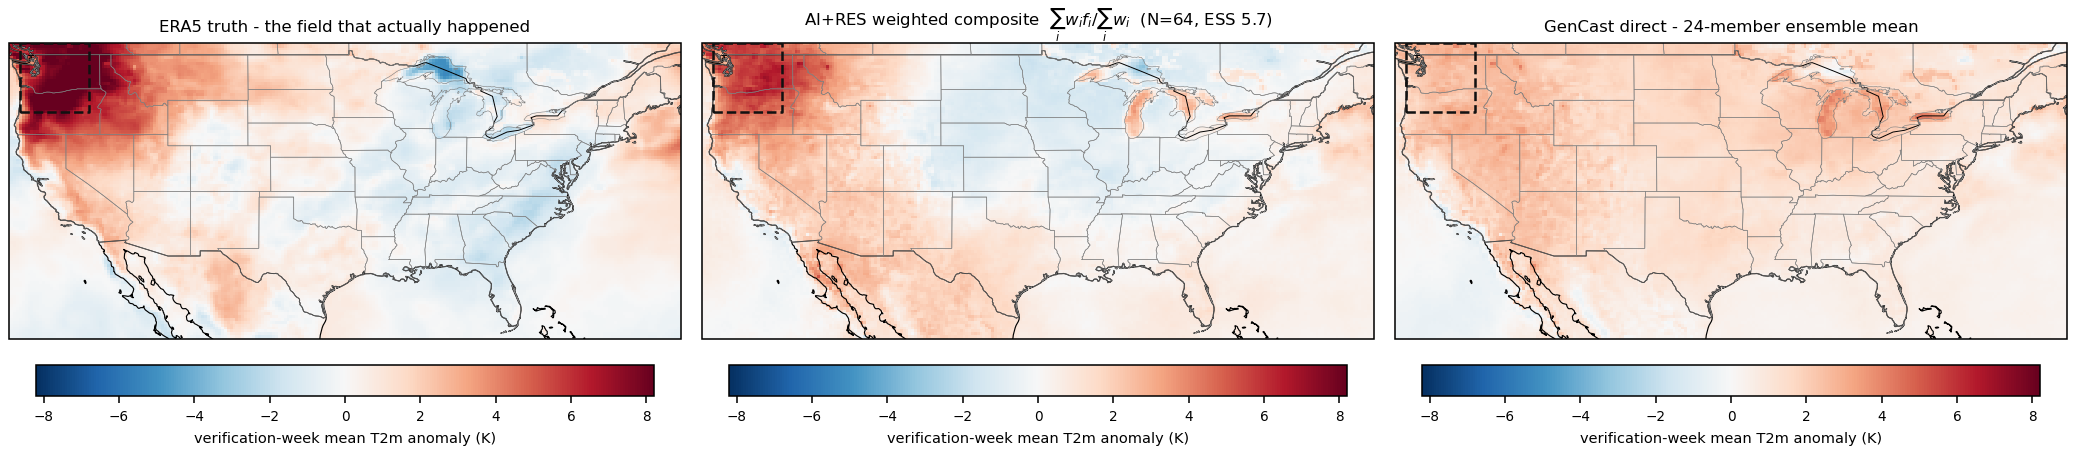
\includegraphics[width=\textwidth]{figs/pnw_anom_maps.png}
\caption{The 2021 heat dome as fields. Left, the ERA5 7-day mean $\Tm$ anomaly over the verification week. Middle, the weighted composite of the 64 resampled walkers, $\sum_i w_i f_i / \sum_i w_i$ with $w_i = e^{-V_K(\text{lineage of } i)}$ and $f_i$ the walker's verification-week field, with a weight ESS of 5.7. Right, the 24-member direct GenCast ensemble mean. Dashed box is the scored region. The composite shows where the estimator's weight is concentrated and is not a forecast. The direct mean has no dome at all.}
\label{fig:maps}
\end{figure*}

\begin{figure*}[tp]
\centering
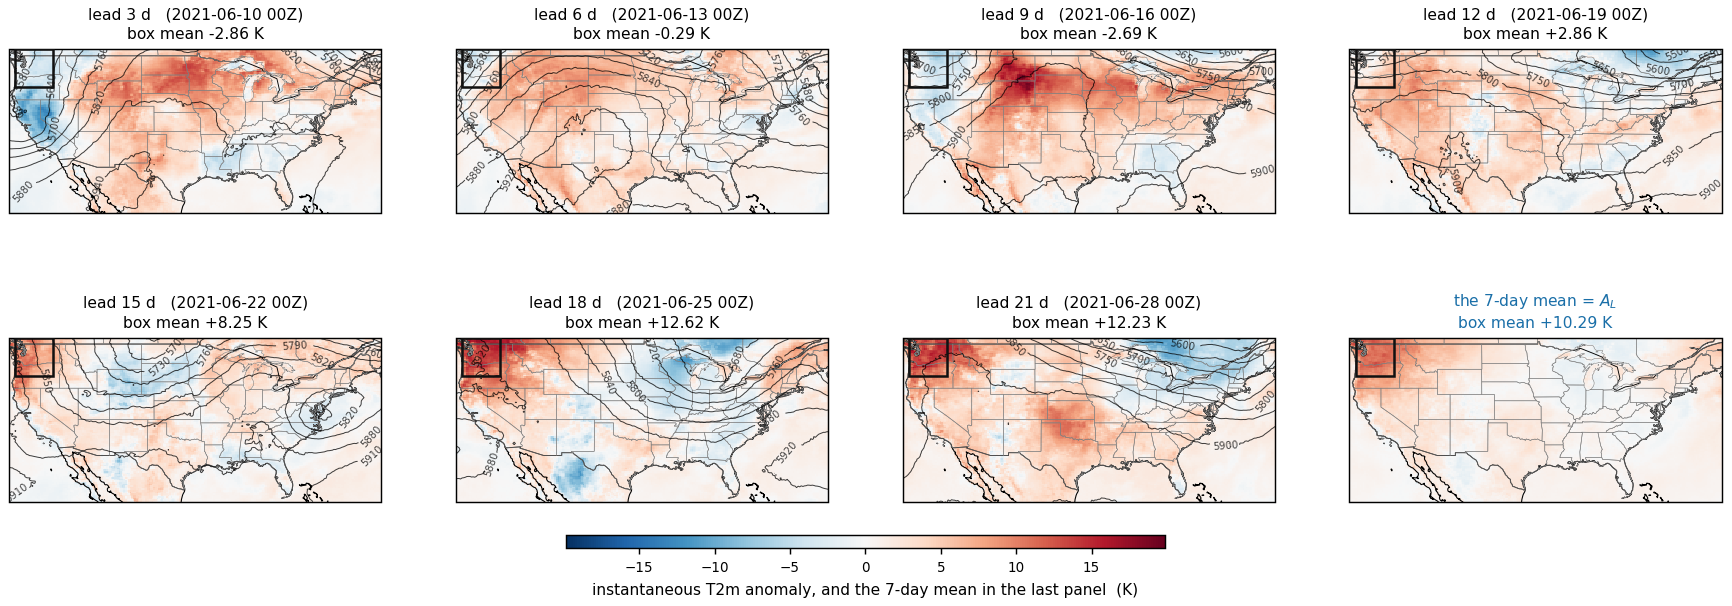
\includegraphics[width=\textwidth]{figs/pnw_map_walk.png}
\caption{The most extreme surviving lineage of the heat-dome run in space, at each barrier, at 18 d and at the peak. Shading is the instantaneous $\Tm$ anomaly and contours are 500 hPa geopotential height from the same walker. The last panel is the 7-day mean that $\AL$ is taken over. At the 9-day barrier this lineage had the fourth-coolest current box anomaly of the 64 alive (\SI{-2.69}{K}) and would have been near the bottom of a persistence ranking. FCN3 ranked it tenth and it drew eleven children, the maximum at that barrier, because the ridge was already building offshore while the surface beneath it had not warmed.}
\label{fig:walk}
\end{figure*}

\paragraph{Maps.}
The box mean cannot distinguish a real dome from a displaced ridge that scores the same number, so every field was reduced on the same grid and compared to ERA5 over the box. The unweighted mean of the 64 resampled walkers (not shown) is the closest field to what happened, with a box root-mean-square error of \SI{0.86}{K}, against \SIrange{5.3}{5.5}{K} for the three baseline ensemble means. That is not a skill claim. The population was aimed at this event, so its mean is not a forecast mean. It says that the observed event lies inside the resampled distribution rather than at its edge. \Cref{fig:maps} shows the same thing for the weighted composite against ERA5 and against the direct GenCast mean, which contains no dome. The far tail overshoots the event, with the top-10 composite \SI{2.3}{K} warmer than ERA5 over the box, as an algorithm that selects on $\AL$ should. \Cref{fig:walk} follows the hottest lineage through the barriers. The 500 hPa ridge that carries the dome is visible to the scorer while the surface anomaly is still below the population mean, which is the single-walker picture of the gate correlations in \cref{sec:impl}, where the FCN3 score has skill from 6 days and the persistence score only from 15.

\paragraph{The operational baseline.}
The dashed curves in \cref{fig:traj_pnw,fig:traj_uri,fig:traj_elliott,fig:traj_sw} are the four 6-hourly CFSv2 cycles ending at the initialisation, so no member is at a shorter lead than the walkers. CFSv2 reaches the observed value on none of the six regional events and on three of the six its ensemble mean is within \SI{1}{K} of climatology. It does reach the two mild CONUS controls. Passing the ERA5 truth field through CFSv2's coarser grid and back changes the box anomaly by at most \SI{0.06}{K} on the six regional events and \SI{0.13}{K} on any of the nine, so the grid is not what is being compared.

\section{Limitations}
\label{sec:limits}

The reach boundary near 3 standard deviations is a property of $N = 64$, $K = 5$ and a $\ck$ schedule capped at 2.0, and the sampler arrives there with the resampling ESS already down to 11 to 18\% of $N$ on the two deepest warm targets. Pushing harder with this $N$ collapses the population. Pushing with a larger $N$ costs linearly. Clone correlation is the mechanism behind both the collapse and the tight spread of the resampled population, whose box standard deviation of \SI{1.8}{K} compares to \SIrange{2.9}{3.3}{K} for the free ensembles. The estimator's factor-of-two scatter in absolute level, its small weight effective sample size and the residual tail bias of the weighted mean are all consequences of the same small $N$ and are stated with each number in \cref{sec:results}. The observable is one scalar per event, a box-mean weekly temperature, chosen because it is the quantity the paper studied and the one the direct ensembles could be compared on. Nine events with a fixed schedule are enough to show the method reaches and prices, and not enough to show its probabilities are calibrated as forecasts, which is the subject of \cref{sec:future}.

\section{Future work}
\label{sec:future}

\paragraph{Other walkers and scorers.}
Nothing in the DMC core knows what a walker is. The same loop that drives GenCast was validated against an Ornstein--Uhlenbeck process with an analytic answer, and the two model roles are behind one interface each. A walker exposes a global two-frame state and a segment roll. A scorer exposes an $M$-member forecast of the observable from that state. A better walker or a better scorer replaces the current one without touching the resampling, the estimator or the figures, provided the hardware can hold it. The present pair needs an 80 GB H100 per card. FCN3 peaks near \SI{50}{GiB} and runs out of memory on a 40 GB A100, and the 0.25\si{\degree} walker fits a 40 GB card only in a serial bfloat16 path at about \SI{80}{s} per step. A 1\si{\degree} walker or a lighter scorer would relax both.

\paragraph{A hurricane score.}
Every event in \cref{tab:slate} is a temperature event. Tropical cyclones were evaluated on the same 7-day box-mean reduction applied to 850 hPa wind speed and rejected. A weekly box mean washes out a one-day landfall, and for Hurricane Ian the observation lands 0.6 standard deviations below the direct ensemble mean, with 17 of 24 direct members already exceeding it. That is a statement about the observable, not the sampler. A score function that targets the cyclone itself, built on a peak-intensity or track-proximity observable that the scorer can forecast at the barrier leads, is in development. The DMC loop, the adapter and the driver are unchanged by it. Only the reduction that turns a forecast cube into $\theta$ and the truth field it is verified against are new.

\paragraph{A hindcast calibration campaign.}
A probability for one event cannot be shown to be right. A population of them can. A 42-case slate of CONUS-wide 7-day anomaly episodes over 2021 to 2025, selected by a written rule rather than curated (31 warm, 11 cold, nesting to 12 cases at \SI{3}{K} and 5 at \SI{4}{K}), has been built at 21-day lead with every initial state staged. Each case is budgeted at $N = 32$ for about \SI{32}{H100\,h}. The walker half measured \SI{17.5}{H100\,h} per case and the score half has not yet been exercised. The 12-case tier at \SI{3}{K} is the first production target. A first leg has been rolled on three cases, one of them partially, after an allocator failure on the shared GPU nodes was worked around. The workaround has passed on the case that previously failed on every attempt, but has no negative control yet. The deliverable is a reliability diagram of the weighted exceedance probability against the observed outcome for the CONUS-mean observable. That slate is not a heat-wave population. Twenty-two of its 42 episodes are in winter and one is in summer, because a regional dome cannot move a CONUS-wide mean by \SI{2}{K}, and the 2021 Pacific Northwest dome is absent from it. Calibrating the regional-box events of \cref{tab:slate} needs the box-level case scan, whose declustering rule currently over-counts and has not yet been fixed.

\section*{Data and code}
The walker, adapter, scorer and resampling core are under \texttt{aires/} on the \texttt{aires} branch of the project repository, and the calibration campaign under \texttt{acal/}. Every figure here is drawn from artifacts written by the run driver and can be regenerated without a GPU. The reference implementation of \citet{lancelin2026airres} is at \url{https://github.com/amaurylancelin/AI-RES-public}.

\bibliography{refs}

\end{document}
